\documentclass[tikz,border=12pt]{standalone}
\usepackage{tikz}
\usetikzlibrary{shapes,arrows.meta,positioning}
\usepackage{amsmath,amssymb}
\usepackage{times}

\begin{document}
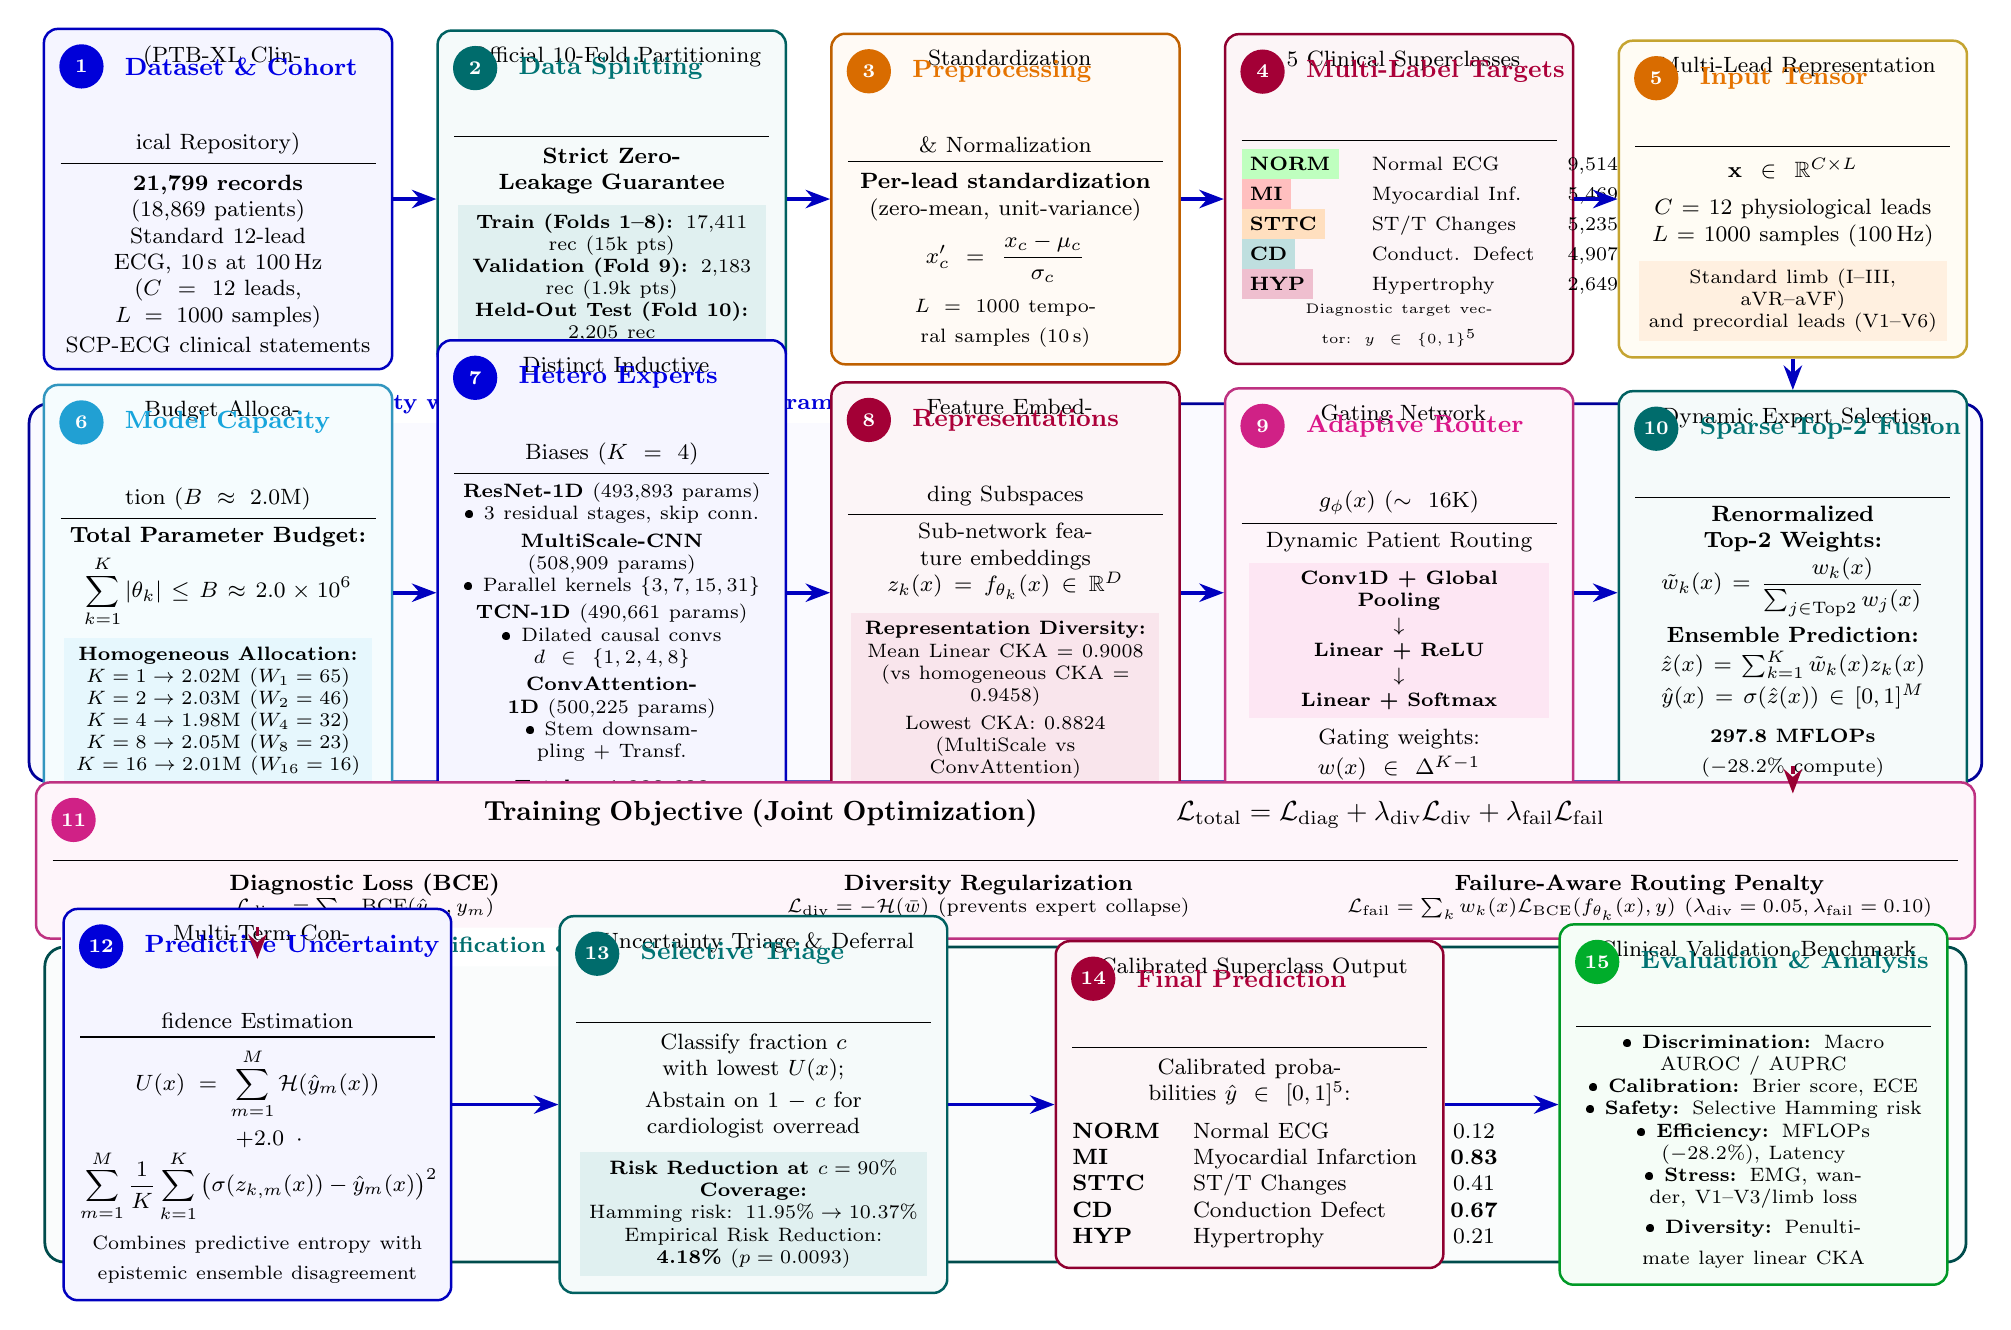
\begin{tikzpicture}[
    font=\small,
    >=Stealth,
    box/.style={
        rectangle, 
        rounded corners=5pt, 
        draw=#1!75!black, 
        fill=#1!4, 
        line width=0.9pt, 
        inner sep=6pt, 
        align=center
    },
    badge/.style={
        circle, 
        fill=#1!85!black, 
        text=white, 
        font=\bfseries\scriptsize, 
        inner sep=0pt, 
        minimum size=16pt,
        align=center
    },
    titletext/.style={
        font=\bfseries\small, 
        text=#1!90!black, 
        anchor=west,
        align=left
    },
    arr/.style={
        ->, 
        line width=1.3pt, 
        draw=blue!75!black
    },
    dasharr/.style={
        ->, 
        dashed, 
        line width=1.3pt, 
        draw=purple!80!black
    },
    frame/.style={
        rectangle, 
        rounded corners=7pt, 
        draw=#1!60!black, 
        fill=#1!2, 
        line width=1.0pt
    }
]

% =========================================================================
% TIER 1: DATA INGESTION & PARTITIONING (y = 12.0)
% 5 boxes: centers at x = 0, 5, 10, 15, 20. Width = 4.3cm, Height = 3.6cm.
% =========================================================================

% Box 1: Dataset & Cohort
\node[box=blue, minimum width=4.3cm, minimum height=3.6cm, text width=4.0cm] (b1) at (0, 12.0) {
    \vspace{22pt}
    \footnotesize (PTB-XL Clinical Repository)\\[3pt]
    \hrule height 0.4pt\vspace{4pt}
    \footnotesize
    \textbf{21,799 records} (18,869 patients)\\
    Standard 12-lead ECG, 10\,s at 100\,Hz\\
    ($C=12$ leads, $L=1000$ samples)\\
    SCP-ECG clinical statements
};
\node[badge=blue] (badge1) at ([xshift=14pt, yshift=-14pt]b1.north west) {1};
\node[titletext=blue] at ([xshift=4pt]badge1.east) {Dataset \& Cohort};

% Box 2: Patient-Stratified Split
\node[box=teal, minimum width=4.3cm, minimum height=3.6cm, text width=4.0cm] (b2) at (5.0, 12.0) {
    \vspace{22pt}
    \footnotesize Official 10-Fold Partitioning\\[3pt]
    \hrule height 0.4pt\vspace{4pt}
    \footnotesize
    \textbf{Strict Zero-Leakage Guarantee}\\[3pt]
    \colorbox{teal!12}{\parbox{3.7cm}{\centering \scriptsize
        \textbf{Train (Folds 1--8):} 17,411 rec (15k pts)\\
        \textbf{Validation (Fold 9):} 2,183 rec (1.9k pts)\\
        \textbf{Held-Out Test (Fold 10):} 2,205 rec
    }}
};
\node[badge=teal] (badge2) at ([xshift=14pt, yshift=-14pt]b2.north west) {2};
\node[titletext=teal] at ([xshift=4pt]badge2.east) {Data Splitting};

% Box 3: Preprocessing & Normalization
\node[box=orange, minimum width=4.3cm, minimum height=3.6cm, text width=4.0cm] (b3) at (10.0, 12.0) {
    \vspace{22pt}
    \footnotesize Standardization \& Normalization\\[3pt]
    \hrule height 0.4pt\vspace{4pt}
    \footnotesize
    \textbf{Per-lead standardization}\\
    (zero-mean, unit-variance)\\[4pt]
    $\displaystyle x_c' = \frac{x_c - \mu_c}{\sigma_c}$\\[5pt]
    \scriptsize $L=1000$ temporal samples (10\,s)
};
\node[badge=orange] (badge3) at ([xshift=14pt, yshift=-14pt]b3.north west) {3};
\node[titletext=orange] at ([xshift=4pt]badge3.east) {Preprocessing};

% Box 4: Multi-Label Targets
\node[box=purple, minimum width=4.3cm, minimum height=3.6cm, text width=4.0cm] (b4) at (15.0, 12.0) {
    \vspace{22pt}
    \footnotesize 5 Clinical Superclasses\\[3pt]
    \hrule height 0.4pt\vspace{3pt}
    \scriptsize
    \begin{tabular}{@{}llr@{}}
        \colorbox{green!25}{\textbf{NORM}} & Normal ECG & 9,514 \\
        \colorbox{red!25}{\textbf{MI}} & Myocardial Inf. & 5,469 \\
        \colorbox{orange!25}{\textbf{STTC}} & ST/T Changes & 5,235 \\
        \colorbox{teal!25}{\textbf{CD}} & Conduct. Defect & 4,907 \\
        \colorbox{purple!25}{\textbf{HYP}} & Hypertrophy & 2,649 \\
    \end{tabular}\\[1pt]
    \tiny Diagnostic target vector: $y \in \{0, 1\}^5$
};
\node[badge=purple] (badge4) at ([xshift=14pt, yshift=-14pt]b4.north west) {4};
\node[titletext=purple] at ([xshift=4pt]badge4.east) {Multi-Label Targets};

% Box 5: Input Tensor
\node[box=yellow!60!orange, minimum width=4.3cm, minimum height=3.6cm, text width=4.0cm] (b5) at (20.0, 12.0) {
    \vspace{22pt}
    \footnotesize Multi-Lead Representation\\[3pt]
    \hrule height 0.4pt\vspace{4pt}
    \footnotesize
    $\mathbf{x} \in \mathbb{R}^{C \times L}$\\[4pt]
    $C = 12\text{ physiological leads}$\\
    $L = 1000\text{ samples (100\,Hz)}$\\[4pt]
    \colorbox{orange!12}{\parbox{3.7cm}{\centering \scriptsize
        Standard limb (I--III, aVR--aVF)\\
        and precordial leads (V1--V6)
    }}
};
\node[badge=orange] (badge5) at ([xshift=14pt, yshift=-14pt]b5.north west) {5};
\node[titletext=orange] at ([xshift=4pt]badge5.east) {Input Tensor};

% Horizontal Flow Tier 1
\draw[arr] (b1.east) -- (b2.west);
\draw[arr] (b2.east) -- (b3.west);
\draw[arr] (b3.east) -- (b4.west);
\draw[arr] (b4.east) -- (b5.west);

% =========================================================================
% TIER 2: EXPERT ENSEMBLE & ADAPTIVE GATING (y = 7.0)
% 5 boxes: centers at x = 0, 5, 10, 15, 20. Width = 4.3cm, Height = 4.2cm.
% =========================================================================

% Enclosing frame drawn directly with coordinates:
\draw[frame=blue] (-2.4, 4.6) rectangle (22.4, 9.4);
\node[font=\footnotesize\bfseries, text=blue!85!black, fill=white, inner sep=3pt, rounded corners=2pt, anchor=west] at (-2.2, 9.4) {Expert Ensemble (Multiplicity with Fixed Budget $\approx$ 2.0M Parameters)};

% Box 6: Capacity Allocation
\node[box=cyan, minimum width=4.3cm, minimum height=4.2cm, text width=4.0cm] (b6) at (0, 7.0) {
    \vspace{22pt}
    \footnotesize Budget Allocation ($B \approx 2.0\text{M}$)\\[3pt]
    \hrule height 0.4pt\vspace{3pt}
    \footnotesize
    \textbf{Total Parameter Budget:}\\[2pt]
    $\displaystyle\sum_{k=1}^K |\theta_k| \le B \approx 2.0 \times 10^6$\\[3pt]
    \colorbox{cyan!10}{\parbox{3.7cm}{\centering \scriptsize
        \textbf{Homogeneous Allocation:}\\
        $K=1 \to 2.02\text{M}$ ($W_1=65$)\\
        $K=2 \to 2.03\text{M}$ ($W_2=46$)\\
        $K=4 \to 1.98\text{M}$ ($W_4=32$)\\
        $K=8 \to 2.05\text{M}$ ($W_8=23$)\\
        $K=16 \to 2.01\text{M}$ ($W_{16}=16$)
    }}
};
\node[badge=cyan] (badge6) at ([xshift=14pt, yshift=-14pt]b6.north west) {6};
\node[titletext=cyan] at ([xshift=4pt]badge6.east) {Model Capacity};

% Box 7: Heterogeneous Architectures
\node[box=blue, minimum width=4.3cm, minimum height=4.2cm, text width=4.0cm] (b7) at (5.0, 7.0) {
    \vspace{22pt}
    \footnotesize Distinct Inductive Biases ($K=4$)\\[3pt]
    \hrule height 0.4pt\vspace{3pt}
    \scriptsize
    \textbf{ResNet-1D} (493,893 params)\\
    \textbullet~3 residual stages, skip conn.\\[2pt]
    \textbf{MultiScale-CNN} (508,909 params)\\
    \textbullet~Parallel kernels $\{3, 7, 15, 31\}$\\[2pt]
    \textbf{TCN-1D} (490,661 params)\\
    \textbullet~Dilated causal convs $d \in \{1, 2, 4, 8\}$\\[2pt]
    \textbf{ConvAttention-1D} (500,225 params)\\
    \textbullet~Stem downsampling + Transf.\\[2pt]
    \textbf{Total = 1,993,688 params} ($+0.92\%$)
};
\node[badge=blue] (badge7) at ([xshift=14pt, yshift=-14pt]b7.north west) {7};
\node[titletext=blue] at ([xshift=4pt]badge7.east) {Hetero Experts};

% Box 8: Feature Representations
\node[box=purple, minimum width=4.3cm, minimum height=4.2cm, text width=4.0cm] (b8) at (10.0, 7.0) {
    \vspace{22pt}
    \footnotesize Feature Embedding Subspaces\\[3pt]
    \hrule height 0.4pt\vspace{3pt}
    \footnotesize
    Sub-network feature embeddings\\
    $z_k(x) = f_{\theta_k}(x) \in \mathbb{R}^D$\\[4pt]
    \colorbox{purple!10}{\parbox{3.7cm}{\centering \scriptsize
        \textbf{Representation Diversity:}\\
        Mean Linear CKA = 0.9008\\
        (vs homogeneous CKA = 0.9458)\\[2pt]
        Lowest CKA: 0.8824\\
        (MultiScale vs ConvAttention)
    }}
};
\node[badge=purple] (badge8) at ([xshift=14pt, yshift=-14pt]b8.north west) {8};
\node[titletext=purple] at ([xshift=4pt]badge8.east) {Representations};

% Box 9: Adaptive Router
\node[box=magenta, minimum width=4.3cm, minimum height=4.2cm, text width=4.0cm] (b9) at (15.0, 7.0) {
    \vspace{22pt}
    \footnotesize Gating Network $g_\phi(x)$ ($\sim 16\text{K}$)\\[3pt]
    \hrule height 0.4pt\vspace{3pt}
    \footnotesize
    Dynamic Patient Routing\\[3pt]
    \colorbox{magenta!10}{\parbox{3.6cm}{\centering \scriptsize
        \textbf{Conv1D + Global Pooling}\\[1pt]
        $\downarrow$\\[1pt]
        \textbf{Linear + ReLU}\\[1pt]
        $\downarrow$\\[1pt]
        \textbf{Linear + Softmax}
    }}\\[3pt]
    \footnotesize Gating weights: $w(x) \in \Delta^{K-1}$
};
\node[badge=magenta] (badge9) at ([xshift=14pt, yshift=-14pt]b9.north west) {9};
\node[titletext=magenta] at ([xshift=4pt]badge9.east) {Adaptive Router};

% Box 10: Sparse Top-2 Routing & Fusion
\node[box=teal, minimum width=4.3cm, minimum height=4.2cm, text width=4.0cm] (b10) at (20.0, 7.0) {
    \vspace{22pt}
    \footnotesize Dynamic Expert Selection\\[3pt]
    \hrule height 0.4pt\vspace{3pt}
    \footnotesize
    \textbf{Renormalized Top-2 Weights:}\\[1pt]
    $\tilde{w}_k(x) = \dfrac{w_k(x)}{\sum_{j \in \text{Top2}} w_j(x)}$\\[3pt]
    \textbf{Ensemble Prediction:}\\[1pt]
    $\hat{z}(x) = \sum_{k=1}^K \tilde{w}_k(x) z_k(x)$\\[2pt]
    $\hat{y}(x) = \sigma(\hat{z}(x)) \in [0, 1]^M$\\[3pt]
    \scriptsize \textbf{297.8 MFLOPs} ($-28.2\%$ compute)
};
\node[badge=teal] (badge10) at ([xshift=14pt, yshift=-14pt]b10.north west) {10};
\node[titletext=teal] at ([xshift=4pt]badge10.east) {Sparse Top-2 Fusion};

% Tier 2 Horizontal Flow
\draw[arr] (b6.east) -- (b7.west);
\draw[arr] (b7.east) -- (b8.west);
\draw[arr] (b8.east) -- (b9.west);
\draw[arr] (b9.east) -- (b10.west);

% Vertical connection from Input Tensor (Tier 1) down to Tier 2
\draw[arr] (b5.south) -- (b10.north);

% =========================================================================
% TIER 3: TRAINING OBJECTIVE (y = 3.6)
% Center at (10.0, 3.6), width = 24.6cm, height = 1.6cm
% =========================================================================
\node[box=magenta, minimum width=24.6cm, minimum height=1.6cm, text width=24.2cm] (b11) at (10.0, 3.6) {
    \vspace{8pt}
    \begin{tabular}{@{}l@{\hspace{50pt}}c@{}}
        \hspace{25pt}\textbf{\normalsize Training Objective (Joint Optimization)} &
        \normalsize $\displaystyle \mathcal{L}_{\text{total}} = \mathcal{L}_{\text{diag}} + \lambda_{\text{div}}\mathcal{L}_{\text{div}} + \lambda_{\text{fail}}\mathcal{L}_{\text{fail}}$
    \end{tabular}\\[3pt]
    \hrule height 0.4pt\vspace{3pt}
    \begin{tabular}{p{7.5cm}p{7.5cm}p{8.2cm}}
        \centering \footnotesize \textbf{Diagnostic Loss (BCE)}\\\scriptsize $\mathcal{L}_{\text{diag}} = \sum_m \text{BCE}(\hat{y}_m, y_m)$ &
        \centering \footnotesize \textbf{Diversity Regularization}\\\scriptsize $\mathcal{L}_{\text{div}} = -\mathcal{H}(\bar{w})$ (prevents expert collapse) &
        \centering \footnotesize \textbf{Failure-Aware Routing Penalty}\\\scriptsize $\mathcal{L}_{\text{fail}} = \sum_k w_k(x) \mathcal{L}_{\text{BCE}}(f_{\theta_k}(x), y)$ ($\lambda_{\text{div}}=0.05, \lambda_{\text{fail}}=0.10$)
    \end{tabular}
};
\node[badge=magenta] (badge11) at ([xshift=14pt, yshift=-14pt]b11.north west) {11};

% Connection Tier 2 to Tier 3: from b10.south (y=4.9) down to b11.north (y=4.4)
\draw[dasharr] (20.0, 4.8) -- (20.0, 4.45);

% =========================================================================
% TIER 4: INFERENCE PHASE & SELECTIVE CLASSIFICATION (y = 0.5)
% 4 boxes: centers at x = 0.5, 6.8, 13.1, 19.5. Width = 4.8cm, Height = 3.6cm.
% Gap between boxes = 6.8 - 0.5 - 4.8 = 1.5cm.
% =========================================================================

% Enclosing frame drawn directly with coordinates:
\draw[frame=teal] (-2.2, -1.5) rectangle (22.2, 2.5);
\node[font=\footnotesize\bfseries, text=teal!85!black, fill=white, inner sep=3pt, rounded corners=2pt, anchor=west] at (-2.0, 2.5) {Inference Phase (Selective Classification \& Clinical Decision Support)};

% Box 12: Predictive Uncertainty
\node[box=blue, minimum width=4.8cm, minimum height=3.6cm, text width=4.5cm] (b12) at (0.5, 0.5) {
    \vspace{22pt}
    \footnotesize Multi-Term Confidence Estimation\\[3pt]
    \hrule height 0.4pt\vspace{4pt}
    \footnotesize
    $\displaystyle U(x) = \sum_{m=1}^M \mathcal{H}(\hat{y}_m(x))$\\[3pt]
    $\displaystyle \quad + 2.0 \cdot \sum_{m=1}^M \frac{1}{K}\sum_{k=1}^K \left(\sigma(z_{k,m}(x)) - \hat{y}_m(x)\right)^2$\\[4pt]
    \scriptsize Combines predictive entropy with\\epistemic ensemble disagreement
};
\node[badge=blue] (badge12) at ([xshift=14pt, yshift=-14pt]b12.north west) {12};
\node[titletext=blue] at ([xshift=4pt]badge12.east) {Predictive Uncertainty};

% Box 13: Selective Classification
\node[box=teal, minimum width=4.8cm, minimum height=3.6cm, text width=4.5cm] (b13) at (6.8, 0.5) {
    \vspace{22pt}
    \footnotesize Uncertainty Triage \& Deferral\\[3pt]
    \hrule height 0.4pt\vspace{4pt}
    \footnotesize
    Classify fraction $c$ with lowest $U(x)$;\\[2pt]
    Abstain on $1-c$ for cardiologist overread\\[4pt]
    \colorbox{teal!12}{\parbox{4.2cm}{\centering \scriptsize
        \textbf{Risk Reduction at $c=90\%$ Coverage:}\\
        Hamming risk: $11.95\% \to 10.37\%$\\
        Empirical Risk Reduction: \textbf{4.18\%} ($p=0.0093$)
    }}
};
\node[badge=teal] (badge13) at ([xshift=14pt, yshift=-14pt]b13.north west) {13};
\node[titletext=teal] at ([xshift=4pt]badge13.east) {Selective Triage};

% Box 14: Final Prediction
\node[box=purple, minimum width=4.8cm, minimum height=3.6cm, text width=4.5cm] (b14) at (13.1, 0.5) {
    \vspace{22pt}
    \footnotesize Calibrated Superclass Output\\[3pt]
    \hrule height 0.4pt\vspace{4pt}
    \footnotesize
    Calibrated probabilities $\hat{y} \in [0, 1]^5$:\\[4pt]
    \begin{tabular}{@{}llc@{}}
        \textbf{NORM} & Normal ECG & $0.12$ \\
        \textbf{MI}   & Myocardial Infarction & $\mathbf{0.83}$ \\
        \textbf{STTC} & ST/T Changes & $0.41$ \\
        \textbf{CD}   & Conduction Defect & $\mathbf{0.67}$ \\
        \textbf{HYP}  & Hypertrophy & $0.21$ \\
    \end{tabular}
};
\node[badge=purple] (badge14) at ([xshift=14pt, yshift=-14pt]b14.north west) {14};
\node[titletext=purple] at ([xshift=4pt]badge14.east) {Final Prediction};

% Box 15: Evaluation & Analysis
\node[box=green!60!teal, minimum width=4.8cm, minimum height=3.6cm, text width=4.5cm] (b15) at (19.5, 0.5) {
    \vspace{22pt}
    \footnotesize Clinical Validation Benchmark\\[3pt]
    \hrule height 0.4pt\vspace{3pt}
    \scriptsize
    \textbullet~\textbf{Discrimination:} Macro AUROC / AUPRC\\
    \textbullet~\textbf{Calibration:} Brier score, ECE\\
    \textbullet~\textbf{Safety:} Selective Hamming risk\\
    \textbullet~\textbf{Efficiency:} MFLOPs ($-28.2\%$), Latency\\
    \textbullet~\textbf{Stress:} EMG, wander, V1--V3/limb loss\\
    \textbullet~\textbf{Diversity:} Penultimate layer linear CKA
};
\node[badge=green!60!teal] (badge15) at ([xshift=14pt, yshift=-14pt]b15.north west) {15};
\node[titletext=teal] at ([xshift=4pt]badge15.east) {Evaluation \& Analysis};

% Connection Tier 3 to Tier 4: from b11.south (y=2.8) down to b12.north (y=2.3)
\draw[dasharr] (0.5, 2.75) -- (0.5, 2.35);

% Horizontal Flow Tier 4 (gap = 1.5cm between boxes)
\draw[arr] (b12.east) -- (b13.west);
\draw[arr] (b13.east) -- (b14.west);
\draw[arr] (b14.east) -- (b15.west);

\end{tikzpicture}
\end{document}
